%% 
%% Copyright 2019-2020 Elsevier Ltd
%% 
%% This file is part of the 'CAS Bundle'.
%% --------------------------------------
%% 
%% It may be distributed under the conditions of the LaTeX Project Public
%% License, either version 1.2 of this license or (at your option) any
%% later version. The latest version of this license is in
%%    http://www.latex-project.org/lppl.txt
%% and version 1.2 or later is part of all distributions of LaTeX
%% version 1999/12/01 or later.
%% 
%% The list of all files belonging to the 'CAS Bundle' is
%% given in the file `manifest.txt'.
%% 
%% Template article for cas-dc documentclass for 
%% double column output.

%\documentclass[a4paper,fleqn,longmktitle]{cas-dc}
\documentclass[a4paper,fleqn]{cas-dc}

%\usepackage[authoryear,longnamesfirst]{natbib}
%\usepackage[authoryear]{natbib}
\usepackage[numbers,sort&compress]{natbib}

\usepackage[]{algorithm2e}

\usepackage{algpseudocode}

%%%Author definitions
\def\tsc#1{\csdef{#1}{\textsc{\lowercase{#1}}\xspace}}
\tsc{WGM}
\tsc{QE}
\tsc{EP}
\tsc{PMS}
\tsc{BEC}
\tsc{DE}
%%% 

\begin{document}
\let\ref\Cref 		
\let\eqref\Cref 	
\let\autoref\Cref 	
\let\WriteBookmarks\relax
\def\floatpagepagefraction{1}
\def\textpagefraction{.001}
\shorttitle{Loo Tung Lun et~al. / Engineering Science and Technology, an International Journal}
\footmarks{\url{https://doi.org/xx.xxxx/j.jestch.20xx.xx.xxx}\\
	2215-0986/\begingroup\tiny{©}\endgroup~20xx Karabuk University. Publishing services by Elsevier B.V.\\
	This is an open access article under the CC BY-NC-ND license (\url{http://creativecommons.org/licenses/by-nc-nd/4.0/}).
}

\bookmark[named = FirstPage]{Design and Implementation of Secure Boot Architecture on RISC-V using FPGA} % Title bookmark used in the pdf
%**************** If the title is short, stay on the first line use [mode = short_title] otherwise ******************
%***************************************** use [mode = title] below ***************************************
\title [mode = title]{Design and Implementation of Secure Boot Architecture on RISC-V using FPGA}    

% Title mark notes if desired
%\tnotemark[1,2]

%\tnotetext[1]{This document is the results of the research
%   project funded by the National Science Foundation.}

%\tnotetext[2]{The second title footnote which is a longer text matter
%   to fill through the whole text width and overflow into
%   another line in the footnotes area of the first page.}

\author[1]{Loo, Tung Lun}
\address[1]{School of Electrical and Electronic Engineering, Universiti Sains Malaysia, 14300, Nibong Tebal, Pulau Pinang, Malaysia.}

\author[2]{Mohamad Khairi Ishak}
\address[2]{School of Electrical and Electronic Engineering, Universiti Sains Malaysia, 14300, Nibong Tebal, Pulau Pinang, Malaysia.}

\begin{abstract} 
There are many well-known open-source bootloaders solutions available today such as UEFI/BIOS, Coreboot and Uboot.
Recently, RISC-V as an open-source Instruction Set Architecture, has gained a lot of attention in new embedded products
creation and academic research purpose. In this study, x86, ARM and RISC-V Instruction Set Architecture boot flow and
boot solutions are studied, simulated, experimented, and summarized. Security feature is implemented in firmware and
measured against non-secured firmware to compare boot performance without security inclusion. A new proposed method
to create a security block in Register Transfer Level to generate Secure Hash Algorithms 5 digest is implemented using Field
Programmable Gate Array. The performance of this method is analyzed with the numbers of logic gate required and the
execution time in software versus hardware. As a result of this study, it is observed that in simulated environment, secured
firmware incurred 3.3 Megabytes of additional binary size and 747ms (35 \%) additional boot time compared to non-secured
firmware. A hardware implementation is proposed in Field Programmable Gate Array (FPGA) to reduce the need for a larger
size firmware and longer boot time to implement security. The results of this implementation indicate a requirement of
32,048 gates to implement a SHA512 IP that reduce software execution time by 1132 \%.  
\end{abstract}

% Article history - Should only be set by an editor
\received {27 July 2021}
\revised {xx Month 2021}
\accepted {xx Month 2021}
\online {xx Month 2021}

\begin{keywords}
RISC-V \sep 
Security \sep 
Firmware
\end{keywords}

\maketitle
\section{Introduction}
All compute devices today are powered by a few processors Instruction Set Architectures
(ISAs), predominantly x86, AMD, ARM, and MIPS which is later converged to RISC-V in
2021  \cite{R5:1}. These ISAs provide flexibilities and extensibilities to the
different engineering audiences, creating tremendous opportunities today that benefits
consumer in many custom applications and use cases, especially in the booming edge devices
in Internet of Things world. While having multiple ISA options are good, it is often difficult to
make a good decision on which architecture to go for, because there are many factors that
contribute to design decision. Several key elements of consideration while picking an ISA are as below.

\renewcommand\labelitemi{\small$\bullet$} % Change the size of the bullets in itemize
\begin{itemize} 
\itemsep=-1pt 		% Item separation between items
\itemindent=-3pt 	% Extra indentation from the left margin if necessary
\item 
Time-To-Market (TTM) \\ \\
The TTM factor is about how easy it is to enable an embedded system with collaterals
provided by the ISA provider. For example, the development time of an engineering team
(often called OEM/ODM) taking a new 11th Generation Intel chip and providing a full
solution with it. Several key factors that directly impact TTM are the availabilities of
documentation, system level open-source references and manufacturing technology.
\\

\item 
Cost \\ \\
This factor includes cost of licensing, software, and hardware development cost that the
OEM/ODM needs to pay to get the products released.
\\

\item 
Design flexibilities \\ \\
The design flexibilities revolve around two key questions of “How easy it is to include a
new custom IP in a new design?” and “How easy it is to land firmware, driver, and
software support of a new IP?"
\end{itemize}

An ideal SOC would not only needs to be functional, but also be protected since the very early
initialization flow to ensure no malicious code can be injected at any point before arriving at
user space applications. To achieve this, firmware architecture becomes an important topic
of exploration to identify the security scheme offered with different ISA and how a generic
security approach can be deployed to implement security in each of them. The gap of today’s
security scheme is the ease of deployment whereby the enablers and users would often end up
disabling security just to improve the performance of the system, reduce the TTM and product price.
The consequence of this problem will be more unsecured devices being in the market,
causing risks to everyone in the IOT chain. Therefore, this research will focus on identifying the
boot elements of each ISA, methodology to enable secure boot, and how a security IP block
can be added to the register transfer and firmware level to facilitate security such that it
does not significantly jeopardize system performance and is easy to enable without much
additional software development.

The key objective identified for this research is to
evaluate the secure firmware feature, measure it against boot performance, and propose
security enhancement through Field Programmable Gate Array (FPGA) for firmware booting
mechanism with the evaluated security features of an open-source ISA. This enhancement
could be potentially scale to close-source ISA.

In this paper, section 1 describes the introduction, problems and objectives of the study.
Section 2 describes the background and previous work related to RISC-V processor, boot flow, and
security. Section 3 describes the proposed method, which includes secure boot in Software (QEMU)
and hardware implementation through FPGA. Section 4 describes the experimental setup results and
discussion. Section 5 concludes the study and identify future improvement opportunities.

\section{ Background and previous work}

\subsection{ RISC-V processor and security}
RISC-V boot flow consists of ROM, loader, runtime, boot loader and OS, which aligns to the RISC processor modes that go from the most privileged mode to the least privileged mode as Figure 1 demonstrated. 

\begin{figure}[hbt!]
	\centering
	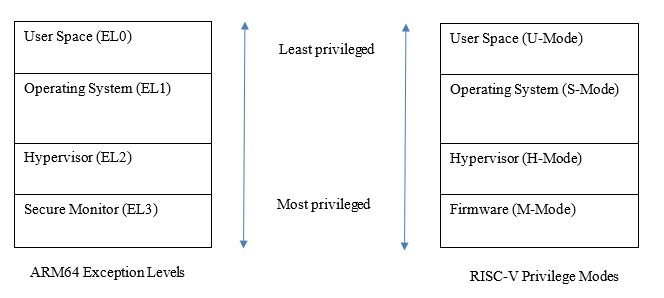
\includegraphics[width=0.5\textwidth,height=2in]{figs/ArmAndRiscVProcessorModesComparison.JPG}
	\caption{ARM and RISC-V Processor Modes Comparison}
\end{figure}

Figure 1 also shows that all stages (Firmware, Hypervisor, OS, User space) are executed in sequence of exception levels like ARM64 fashion. ARM’s EL3 has platform specific runtime firmware and has secure privileges, while RISC-V’s M mode has platform specific firmware only and does not have secure privilege. ARM started with EL3, which is a secure world, while RISC-V starts from M mode, which is a bare metal machine code. The non-secure bootloaders in ARM uses ARM trusted firmware to switch to EL2, while RISC-V uses OpenSBI to switch into S-Mode from M-Mode. Also, ARM is close source while RISC-V is open source. Therefore, due to the open-source nature of RISC-V, the firmware stages between ROM code and OS (kernel space) are extremely flexible.

\begin{figure}[hbt!]
	\centering
	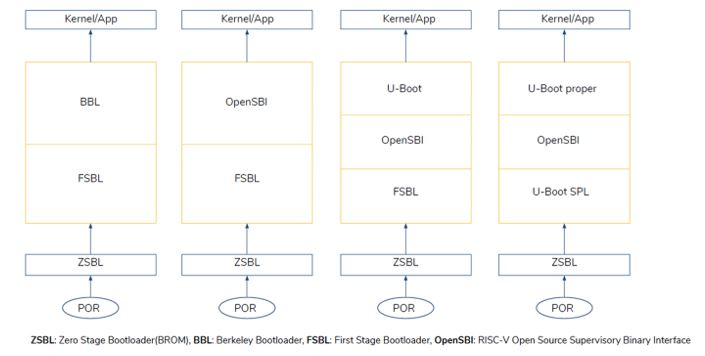
\includegraphics[width=0.5\textwidth,height=2in]{figs/DifferentFirmwareFlowsForRiscV.JPG}
	\caption{Different Firmware Flows For RISC-V \cite{R51:1}}
\end{figure}

Figure 2 shows some examples of different combinations possible after the “Zero stage Bootloader BROM”, such that it contains a combination of U-boot, First Stage Bootloader, OpenSBI (RISC-V Open-Source supervisory binary interface) and BBL (Berkeley Bootloader). Even though having huge flexibility is good, this has eventually become a scalability issue if boot flow is not standardized, and all different RISC-V solutions adopt different methodologies. Maintenance and reusing existing source code and framework features become an issue.

Therefore, in 2020, the boot stage is further standardized to use U-Boot and OpenSBI as the only open source accepted methodology. Figure 3 shows the upstream boot flow where OpenSBI sits right in the middle of boot phase between M-mode (firmware) and S-mode (U-boot) to provide all runtime services.

\begin{figure}[hbt!]
	\centering
	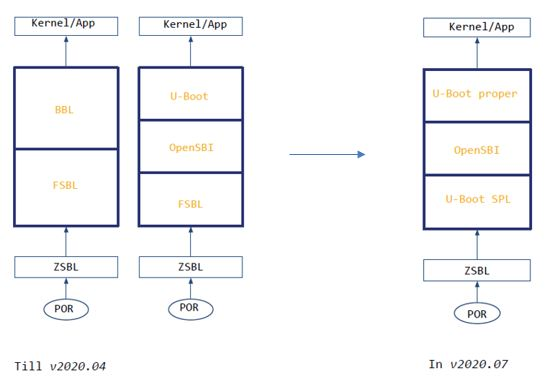
\includegraphics[width=0.5\textwidth,height=3in]{figs/RiscVStandardBootFlow.JPG}
	\caption{RISC-V Standard Boot Flow \cite{R51:1}}
\end{figure}

Figure 3 from Atish et al. also demonstrated that FSBL, which was SiFive specific, will be replaced by Coreboot/U-boot SPL. U-boot will then act as the last stage boot loader before Linux. OpenSBI standard started as an ingredient that is specific only to RISC-V, which makes it important to understand what it does and how it evolved over time. Jagan presented in China RISC-V Forum 2019 shows the evolving of RISC-V Supervisor Binary Interface (SBI) to Open-Source Supervisor Binary Interface (OpenSBI). In summary of the specification changes, the system calls type interface layer between firmware runtime, M mode and S mode were made modular, scalable, and extendable between all CPU and Silicon specific hardware configuration. OpenSBI now contains platform independent and dependent libraries, which support SiFive U540, Andes AE350, Ariane FPGA, Kendryte K210 and QEMU \cite{R51:1}.

The current RISCV boot stage ported to UEFI is initiated by Hewlett Packard Enterprise since 2015  \cite{R51:2}. It described some architectural changes with OpenSBI as a platform structure layer that is callable by services during UEFI boot flow, for example during SEC phase, SEC module would call the OpenSBI initialization and platform initialization code and then return to PEI core once done. In PEI phase, PEI module extracts device tree information constructed in OpenSBI to be further consumed in DXE driver. In DXE and OS run time, supervisor, and hypervisor ecall interface is made available for any run time service required from OpenSBI. This flow is simplified in Figure 4.

\begin{figure}[hbt!]
	\centering
	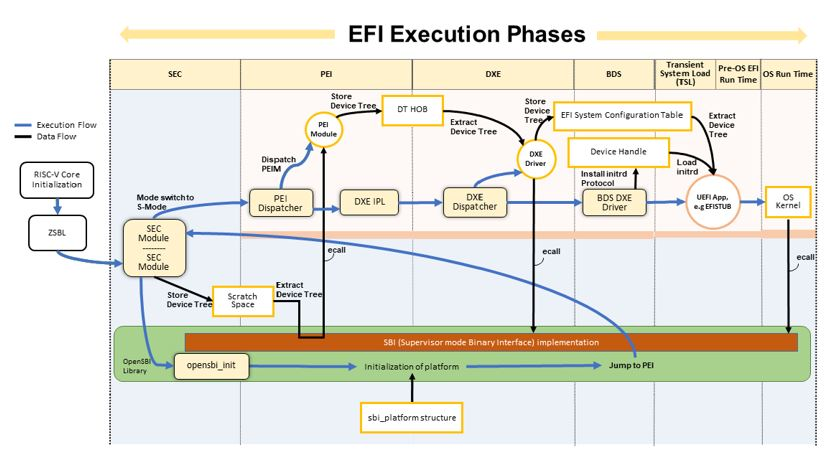
\includegraphics[width=0.5\textwidth,height=2.5in]{figs/HighLevelOverviewOfEfi.JPG}
	\caption{High Level Overview Of EFI Execution Phases with RISC-V \cite{R51:2}}
\end{figure}

The boot phase porting from RISCV essential services to UEFI framework involves more than just adding OpenSBI libraries as another underlayer service. It also entails a volume top file (VTF) that generates a reset vector for UEFI bootloader to jump into, binding processor, converting RISCV ELF format to PE COFF, and porting of other UEFI libraries such as base memory, DXE real time clock, CPU arch, timer arch, reset protocol and CSR (control status registers). A MSCRATCH CSR is used to maintain a V machine mode trap handler in each of the boot phases (SEC, PEI, DXE core). More details of these work in each boot phase are simplified in Figure 5.

\begin{figure}[hbt!]
	\centering
	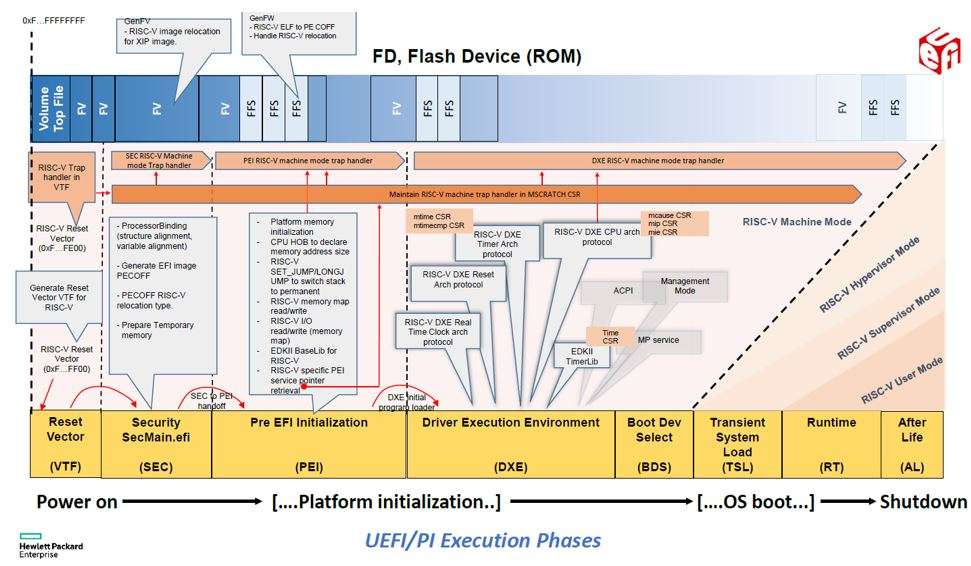
\includegraphics[width=0.5\textwidth,height=2.5in]{figs/RiscVDetailedEfiFlow.JPG}
	\caption{Detailed EFI Execution Phases with RISC-V \cite{R51:2}}
\end{figure}

In RISC-V, two security architectures stood out in addressing the challenges in x86 and ARM world today, namely Sanctum \cite{R5:6} and HECTOR-V \cite{R5:5}. Sanctum provides a similar enclave like concept as Intel SGX. Enclave page table registers and walker/transform logic are added on top of the LLC cache logic. On top of that, it adds measurement root of trust in a temper-resistant hardware. The goal of Sanctum is to target side channel attack that was claimed not covered in Intel SGX. This is achieved by adding page entry transformation logic in Figure 6. Figure 7 further shows the root of trust in the CPU ROM where the code reads security monitor from untrusted flash memory and generate key based on monitor’s hash. The software stack of an enclave is designed in a way that user’s sanctum-aware runtime code and data communicate directly to the security monitor in machine’s measurement root as Figure 8.

\begin{figure}[hbt!]
	\centering
	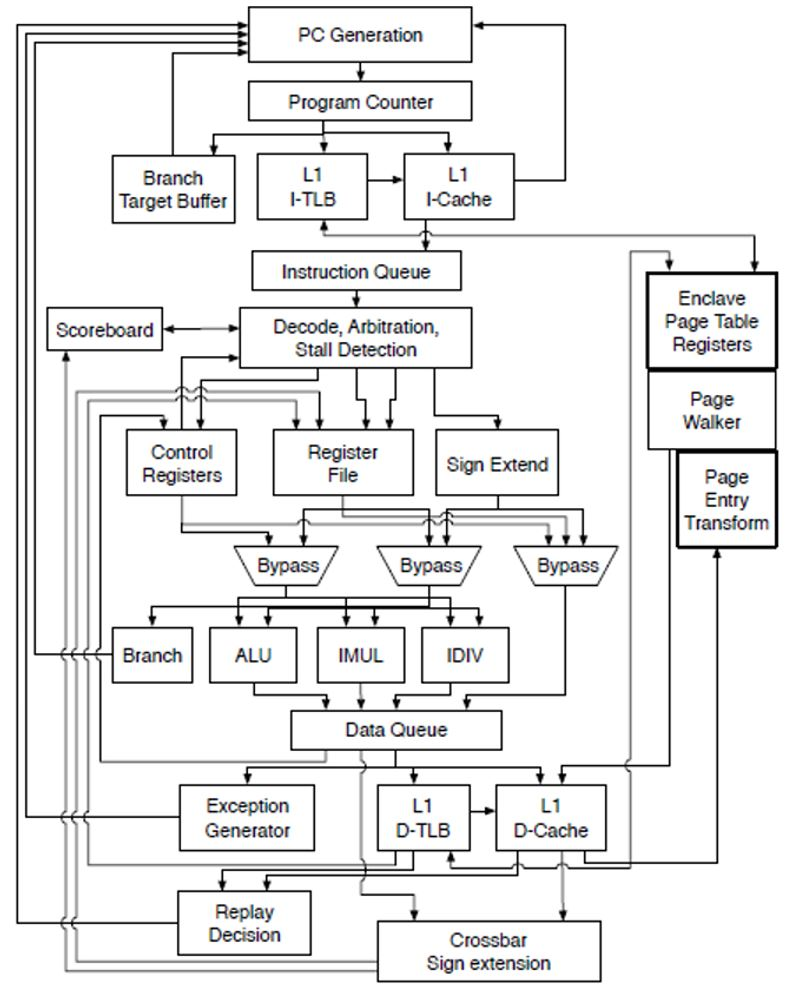
\includegraphics[width=0.5\textwidth,height=4in]{figs/SanctumPageEntryTransformationLogic.JPG}
	\caption{Sanctum Page Entry Transformation Logic in Rocket Core \cite{R5:6}}
\end{figure}

\begin{figure}[hbt!]
	\centering
	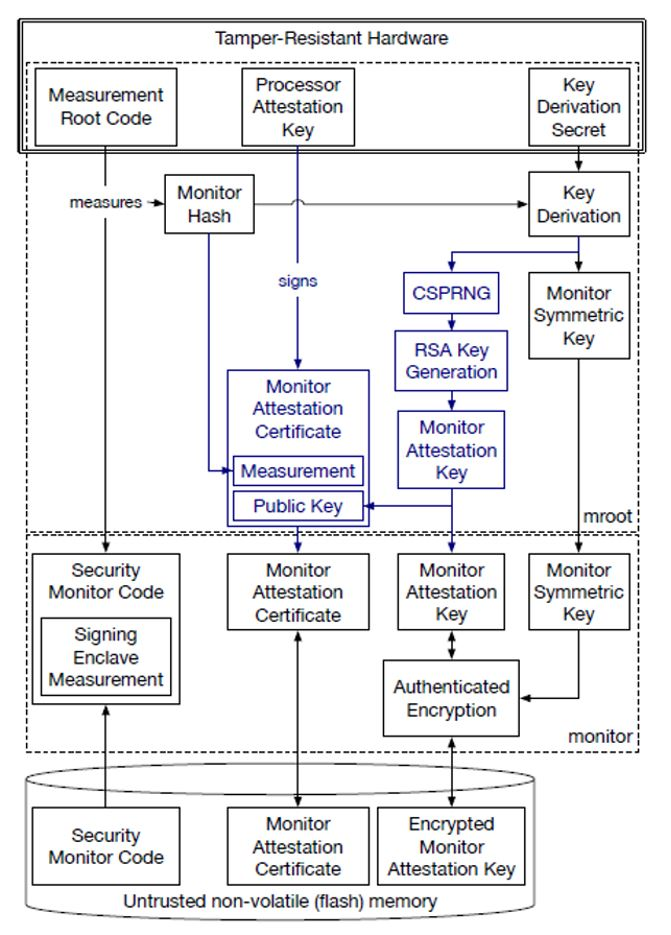
\includegraphics[width=0.5\textwidth,height=3.5in]{figs/SanctumRoT.JPG}
	\caption{Sanctum Root of Trust  \cite{R5:6}}
\end{figure}

\begin{figure}[hbt!]
	\centering
	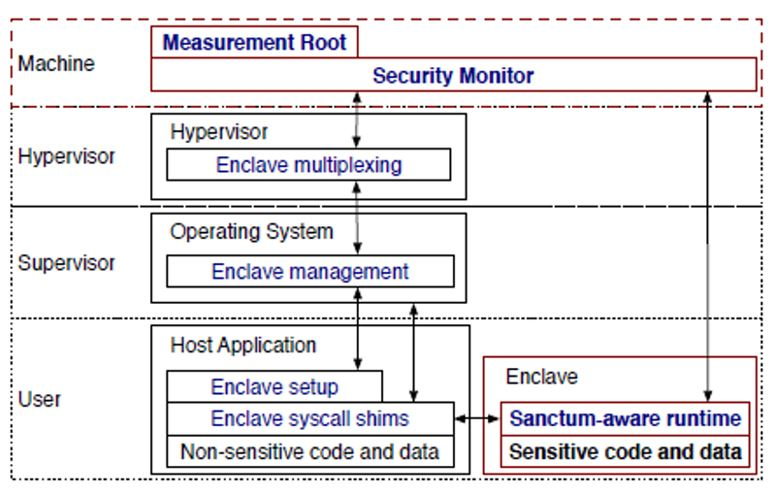
\includegraphics[width=0.5\textwidth,height=2in]{figs/SanctumSwStack.JPG}
	\caption{Sanctum Software Stack TCB  \cite{R5:5}}
\end{figure}

Another popular piece that explores using heterogenous multicore architecture to realize a secure TEE design in RISC-V is HECTOR-V. It has RISC-V Secure Co Processor (RVSCP) embedded to application processor that enable HECTOR-V with mechanism to establish secure communication channels between multiple devices connected to the CPU. Its architecture is described in Figure 9. With this proposed heterogenous architecture, RVSCP provides hardware enforced control flow integrity and restricts I/O accesses to certain execution states. Concurrently, SiFive also developed WorldGuard architecture. In this architecture, each core gets assigned a world ID and process of the core is annotated with process ID. This ID is transported using the interconnect and requests from participants are filtered by peripherals, the memory, and the caches. This is mostly similar to HECTOR-V’s design. The only difference is that WorldGuard transfer the security monitor ownership dynamically to any party for flexible use case, as compared to HECTOR that has concrete secure processor.

\begin{figure}[hbt!]
	\centering
	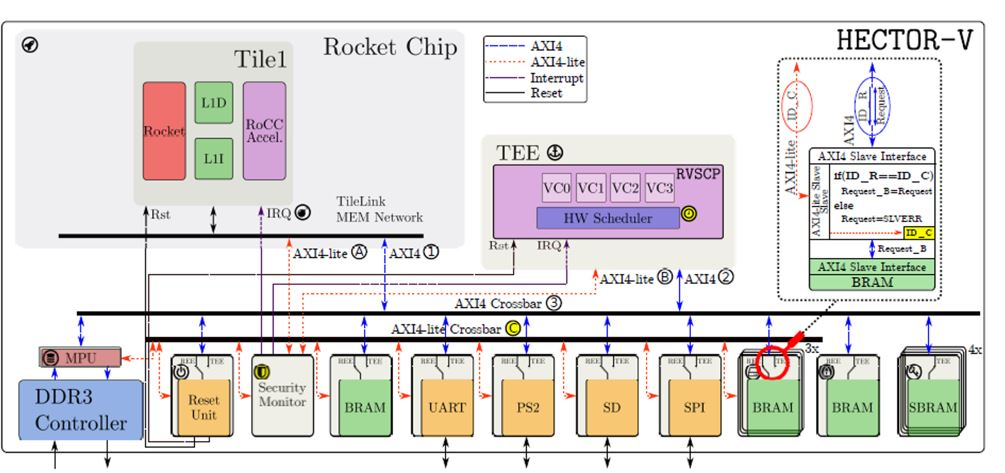
\includegraphics[width=0.5\textwidth,height=1.5in]{figs/Hector.JPG}
	\caption{Hector-V architecture}
\end{figure}

\subsection{ Other related work}
In the past, many researches related to security features available in different ISA had been carried out.
Ning et al analyzed several hardware assisted TEE such as Intel SGX, ARM TrustZone Technology
and AMD SEV, and evaluated the feasibility of deploying them on edge compute infrastructure by evaluating the performance overhead \cite{R5:2}.
More security and performance benchmark study had been carried out by Christian et al and it has been discovered that AMD SEV has the best benchmark with memory protection mechanism at execution speed of near native speed compared to Intel SGX \cite{R5:3}.
Other than performance evaluation, there are also comparative study on multiple ISAs. Geraldine et
al summarized some key challenges of security features, short coming of ARM TrustZone and Intel SGX, and proposed countermeasures in RISC-V architecture that address its defined thread models \cite{R5:4}.
In respective targeted technology domain, Pascal et al proposed HECTOR-V, a RISC-V based architecture to improve on the flexibilities of peripherals’ permission management \cite{R5:5}.Victor et al on the other hand, proposed Sanctum, a RISC-V based TEE to improve on software isolation with comparison to Intel SGX  \cite{R5:6}. There are also several researches that provide deep dive study and survey on existing technologies, for example, Intel SGX was deeply explained from different aspects from the technology use cases to vulnerabilities by Victor et al \cite{R5:7}, an ARM TrustZone comprehensive survey was carried out by Sandro et al \cite{R5:8} and multiple System Management Mode usage model for security purposes was analyzed by William in his PHD report \cite{R5:9}. The researchers work is summarized in Table 1.

\begin{table}[hbt!]
	\caption{Previous Researchers Work}
	\centering
	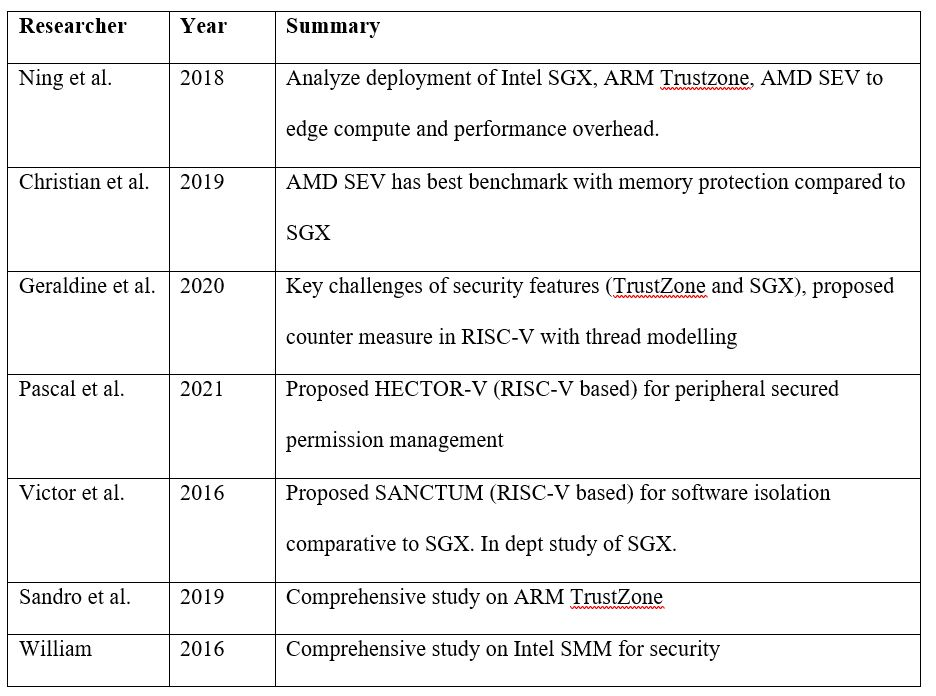
\includegraphics[width=0.5\textwidth,height=2.5in]{figs/PreviousResearchersWork.JPG}
\end{table}

\section{ Proposed Method}
The approach of the research to propose the methodology and collect results is demonstrated in Figure 1. In section 2.1, the platform alternatives are compared and selected. In section 2.2, secure boot implementation is proposed for RISC-V with firmware implementation in software emulated environment (QEMU). In section 2.3, secure boot implementation is proposed for RISC-V with RTL implementation in FPGA hardware environment. In section 2.4, experiments and parameters are proposed to evaluate the firmware and RTL implementation.

\begin{comment}
% Span figure example on double column
\begin{figure}[hbt!]
	\centering
	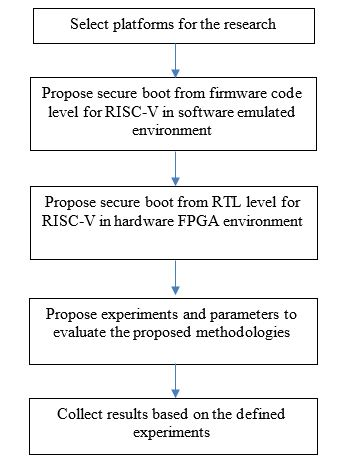
\includegraphics[width=0.35\textwidth,height=2.5in]{figs/ResearchApproach.JPG}
	\caption{Research Approach}
\end{figure}


\subsection{ Platform Selection}
A comparison between software emulation (QEMU), reference boards, and FPGA is created, considering the factor of cost, scalability, availability of resource, and configurability as illustrated in Table 1. As a result of the comparison, QEMU and FPGA are selected for software emulation and hardware enhancement experiment purpose. The QEMU installed is version 6.0.0 on Ubuntu 20.04.2.0 LTS. The FPGA board chosen is Xilinx Nexys A7 DDR4 board with Artix-50T FPGA as Figure 2 because of its affordable price (\$229) and sufficient logic gate for low scale security level exploration. This FPGA is also supported by a few RISC-V projects, such as NEORV32.

\begin{table}[hbt!]
\caption{Platform Comparison}
    \begin{tabular}{|p{0.1\linewidth} | p{0.1\linewidth} | p{0.1\linewidth} | p{0.3\linewidth} | p{0.2\linewidth} |}
        \hline
        Platform & Unit Cost & Scalability & Availability of resources & Configurability \\
        \hline 
        QEMU & None & High & Many firmware solutions support is available on the market as open source.   & High   \\
        \hline
        Reference boards & Low & Low & Different board supports different ISA and different firmware solution. The support comes from OEM and is usually closed source    & Low \\
        \hline
       FPGA & Medium-High & Medium & Several open-source projects are available for RISC-V. However, for x86 and ARM, most of the design is closed source    & High \\
        \hline
    \end{tabular}
\end{table}

% Span figure example on double column
\begin{figure}[hbt!]
	\centering
	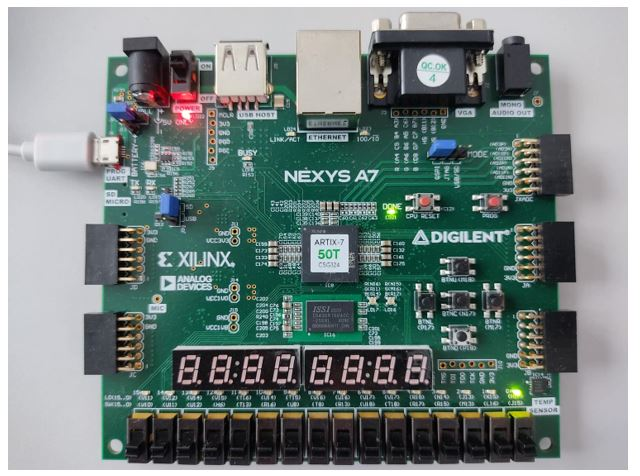
\includegraphics[width=0.5\textwidth,height=2in]{figs/Nexys.JPG}
	\caption{FPGA Selected}
\end{figure}

\end{comment}

\subsection{ Secure Boot in Software/QEMU}
The flow to identify secure boot ingredient has two key flows. The difference between the 2 flows are demonstrated as Figure 10, whereby the firmware is first being compiled and executed without any secure boot ingredient, then showcase how inject secure boot code and execute the firmware. As the firmware code boot stages are compiled as separate binaries, each of the binaries can be then hashed and verified.

Figure 11 describes the potential to apply UEFI secure boot to the existing RISC-V boot with the existing UEFI framework on x86 QEMU. The idea is to inject security stack in UEFI PEI and DXE phase so that the RISCV UEFI boot flow can have secure boot encapsulated. This topic was flagged as a potential enabling item by RISC-V presentation \cite{R5:10}. The security stack by UEFI services had been made available with OpenSSL as the underlayer library and a comprehensive technical report of this describing how to sign and incorporate the keys has been created by \cite{R5:11}. The algorithm to verify the hash of a firmware region is as illustrated as Algorithm 1.

% Span figure example on double column
\begin{figure}[hbt!]
	\centering
	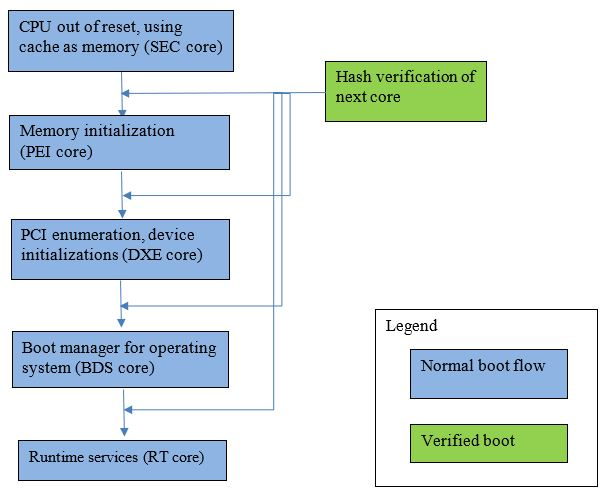
\includegraphics[width=0.5\textwidth,height=3in]{figs/SoftwareSecureBootFlow.JPG}
	\caption{Software Secure Boot Flow}
\end{figure}



\begin{algorithm}
 \caption{Flow illustration of secure boot in firmware}
map the ROM code to a memory region\;
get the memory address pointer and size\;
call SHA512\_INIT()\;
call SHA512\_Update() with the pointer and size\;
call SHA512\_Final() to get the digest.\;
compare the digest with a pre-saved digest in hardware root of trust\;

\eIf{comparison matches}{
   continues the boot process and runs the next firmware code\;
   }{
   halt the boot process due to security violation\;
  }

\end{algorithm}

% Span figure example on double column
\begin{figure}[hbt!]
	\centering
	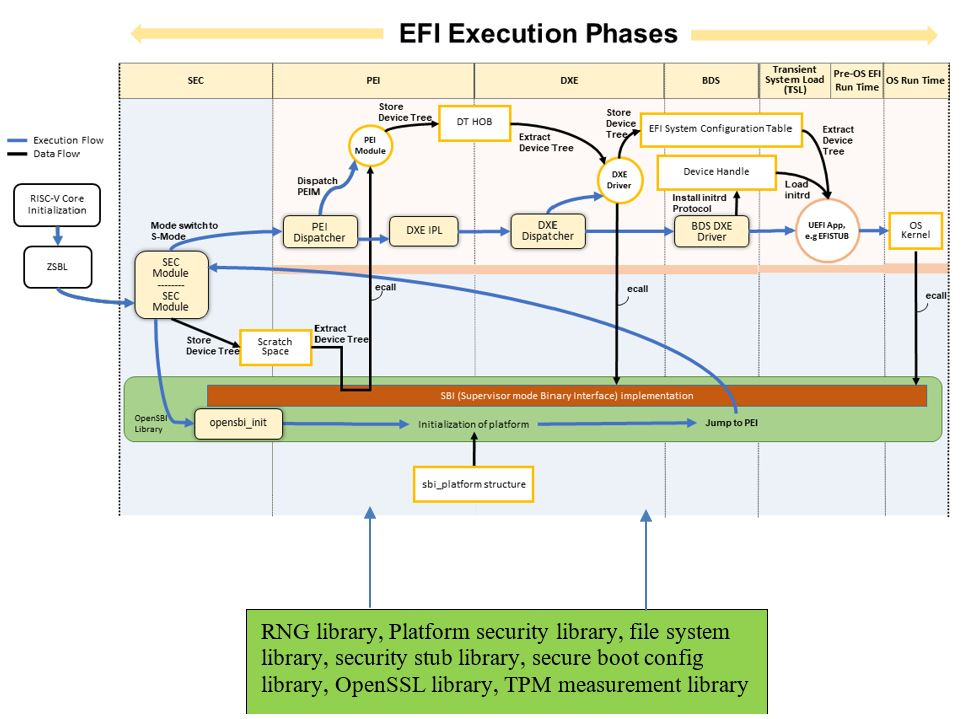
\includegraphics[width=0.5\textwidth,height=3in]{figs/SecureBootOnRISCV.JPG}
	\caption{UEFI Secured Boot on RISC-V}
\end{figure}

\subsection{ Hardware implementation through FPGA}
Another part of the methodology is to propose a method to replace these secure boot services with RTL instead of bootloader code to effectively reduce flash size and improve boot performance. To achieve this, an open-source RISCV processor (NEORV32) is used as an initial environment. SHA512 digest generation block is then added to the RTL of NEORV32, and the digest generated is passed to bootloader via a new read only register block through the custom functions subsystem (CFS) IP. With this implementation, bootloader will no longer need to contain and execute security code to achieve security purpose. A bird-eye view of what is being added is illustrated in green boxes of Figure 12. The IP are customized to introduce an additional arbitration block with state machine that is capable to map the boot rom content to be sent to SHA512 security block to produce digest. Once digest data is produced, the arbitration block will notify custom functions subsystem block with a status complete bit together with 512-bit SHA information. 

% Span figure example on double column
\begin{figure}[hbt!]
	\centering
	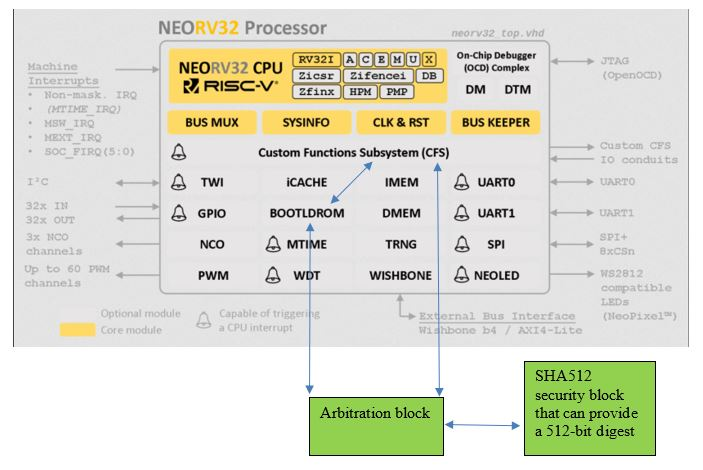
\includegraphics[width=0.5\textwidth,height=2.5in]{figs/HardwareSecureBootBlock.JPG}
	\caption{Hardware Secure Boot Block}
\end{figure}


Figure 13 and figure 14 demonstrates the detailed comparison of system port map after Arbiter and SHA512 core is being added to NEOV32 CPU processor. The details of how the SHA512 core and arbiter block from signals level and how they are being consumed is described subsequently.

Based on the connections shown in Figure 15, during normal boot up process, NEORV32 CPU fetches instructions from bootloader ROM to execute. The amount of memory mapped IO and functionalities depend heavily on how the CPU is connected to data bus and in this case, the custom functions system block. The custom functions system block defines an interface consist of offset of each data that bootloader can read and write data from. The SHA512 Core block is responsible for taking in blocks of data to hash, and then provide output of the digest once completed. Arbiter is the middleman which controls the operation of taking ROM data and send to SHA512 Core to be hashed. Once the hash operation is completed, the digest and the completion status will then be shared with custom functions system to be accessible by CPU, which translate to software accessible registers.

% Span figure example on double column
\begin{figure}[hbt!]
	\centering
	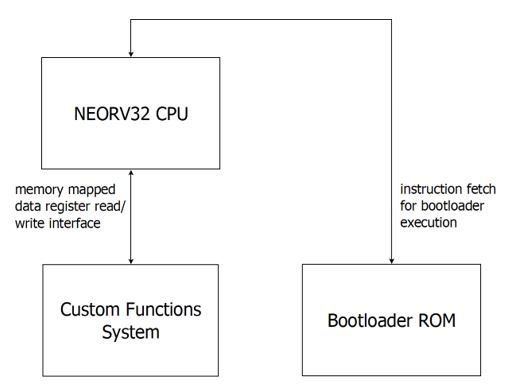
\includegraphics[width=0.4\textwidth,height=1.55in]{figs/SystemPortMap-Original.JPG}
	\caption{System port map of components without security block}
\end{figure}

% Span figure example on double column
\begin{figure}[hbt!]
	\centering
	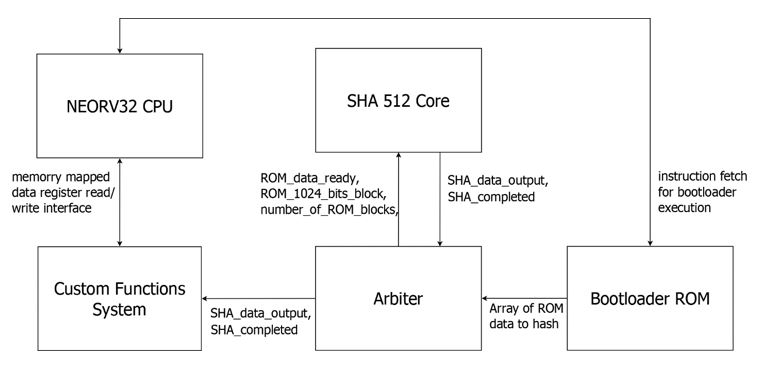
\includegraphics[width=0.4\textwidth,height=1.5in]{figs/SystemPortMap-Amended.JPG}
	\caption{System port map of components to implement additional security block}
\end{figure}


% Span figure example on double column
\begin{figure}[hbt!]
	\centering
	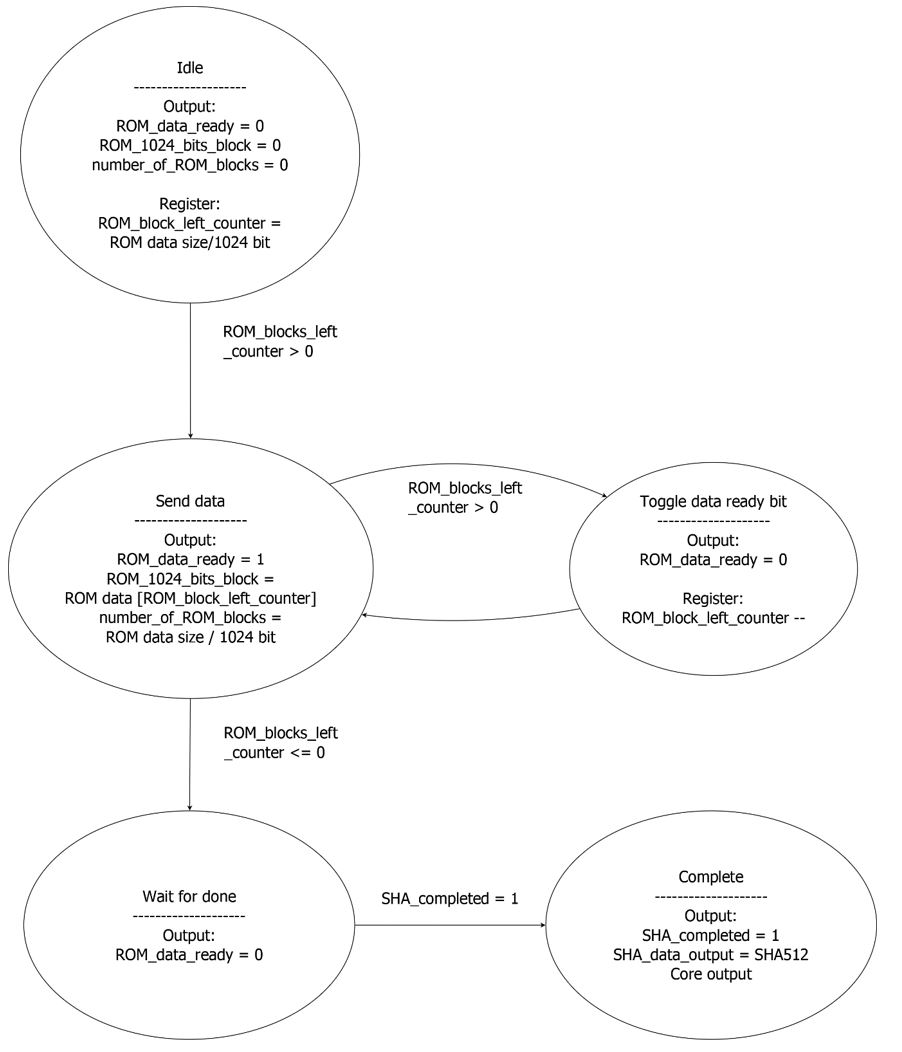
\includegraphics[height=4in]{figs/StateMachine.JPG}
	\caption{State machine of arbitration block}
\end{figure}


The state machine of the arbiter is further designed as Figure 15. It begins with Idle state when everything is initialized to 0. A counter is implemented to keep track of the ROM blocks left to transfer from ROM block to SHA512 core. In send data state, the arbiter will set ROM\_data\_ready for SHA512 block to consume that block of 1024 bits data, then transition to toggle data ready bit state to toggle ROM\_data\_ready bit to 0 and decrement the counter so that the next send data state will transfer next chunk of data to SHA512 core to be processed. Once all blocks had been sent to SHA512 core. It will wait for SHA512 block to respond with SHA\_complete. Once SHA\_complete is set to 1, it will enter a complete state and update the SHA data to custom functions system block together with the SHA\_complete status bit. The algorithm to shift the firmware ROM in sequent to the SHA512 core is as illustrated as Algorithm 2.

\begin{algorithm}
 \caption{Simple illustration of arbitration block}
 \KwData{compiled Bootloader ROM}
 \KwResult{512-bit SHA5 digest}

 \While{not the end of bootloader}{
  shift current 1024-bit bootloader blocks to SHA5\;
  wait for SHA5 block to acknowledge\;
  move to next 1024-bit block\;
 }
\end{algorithm}

\subsection{ Proposed experiments}
The experiment proposed to evaluate the methodology includes 3 parameters.
\begin{enumerate}
\itemsep=-1pt 		% Adjusting item separation
\itemindent=0pt 	% Extra indentation from the left margin if necessary
\item 
Boot performance (time used to boot the firmware)
\item 
Firmware size (size of the compiled binary)
\item 
Number of logic gates consumed in RTL (FPGA resource consumed)
\end{enumerate}

To prove secured boot implementation, negative testing will be performed using unauthorized EFI applications that mimics malicious software to demonstrate that only signed applications can be executed. Therefore, the flow of experiments for software and hardware is planned respectively.

For Software QEMU, a normal unsecured UEFI firmware for x86 and RISC-V is compiled. Then, the UEFI firmware in QEMU is executed by booting to Shell and capturing the boot log.
After this is achieved, a secured UEFI firmware is compiled. Then, the secured UEFI firmware in QEMU is executed by booting to Shell and capturing the boot log.
With the secured UEFI firmware, negative testing is performeced with signed and unsigned EFI application.
The boot time of secured and unsecured firmware are captured. With this and by comparing the results, the impact to boot time after incorporated security can be benchmarked.
The binary size of secured and unsecured firmware are captured. With this and by comparing the results, the impact to firmware binary size after incorporated security can be benchmarked.

For Hardware FPGA, the SHA512 block that interacts with other components in NEORV32 RISC-V processor is implemented.
The SHA512 digest generated by the SHA512 block is captured and compare with the output of software execution to verify the correctness in functionality.
The SHA512 digest generation time is captured to be compared with software execution time to verify the performance.
The boot log of NEORV32 firmware is captured to verify the ability to access SHA512 digest generated by RTL in bootloaders.


\section{ Results/Discussion}
From functional correctness perspective, secured boot is configured as Figure 16. With secure boot enabled, only application software that is being signed with the same keys will be able to execute. To validate this behavior, an unsigned “Hello World” application and a signed “Hello World” application is attempted to execute in EFI Shell environment. Figure 17 shows the unsigned application and Figure 18 shows the signed application. The commit ID used to produce this result is 392836a for efitools repository and 75e9154f81 for EDK2 repository.

% Span figure example on double column
\begin{figure}[hbt!]
	\centering
	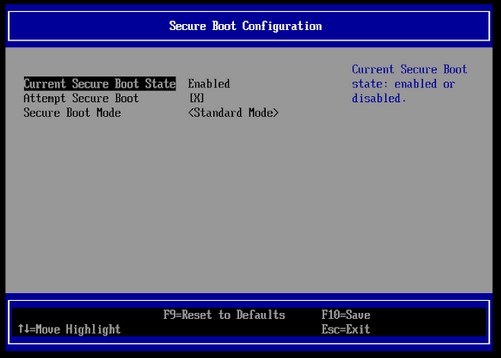
\includegraphics[width=0.5\textwidth,height=3in]{figs/SecureBootConfiguration.JPG}
	\caption{Secure boot configuration}
\end{figure}

% Span figure example on double column
\begin{figure}[hbt!]
	\centering
	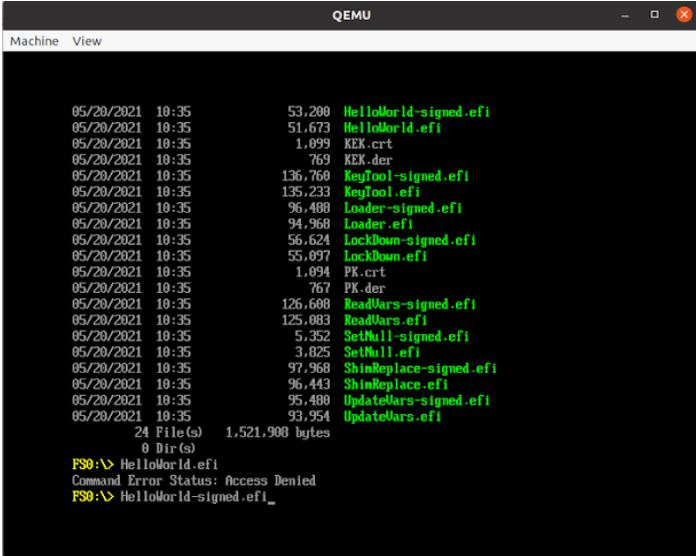
\includegraphics[width=0.5\textwidth,height=3in]{figs/SecureBootUnsigned.JPG}
	\caption{Load unsigned "Hello World" application}
\end{figure}

% Span figure example on double column
\begin{figure}[hbt!]
	\centering
	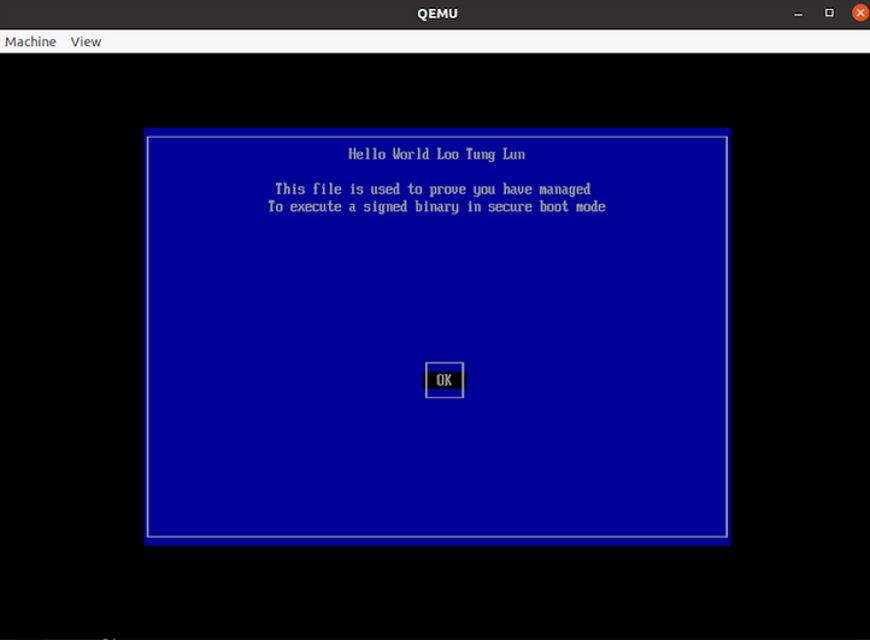
\includegraphics[width=0.5\textwidth,height=3in]{figs/SecureBootSigned.JPG}
	\caption{Loading signed "Hello World" application}
\end{figure}

From firmware size perspective, results collected indicates that non-secure UEFI firmware has a total of 7,602,384 bytes, while secure UEFI firmware has a total of 10,895,864 bytes. Therefore, it is deduced that from software perspective, implementing security in firmware will add additional 3.292 Megabytes (10.895M – 7.602M) of additional binary size.

In terms of boot speed, it is observed that non-secure firmware took 2092 milliseconds to boot while secure firmware took 2839 milliseconds to boot in QEMU. Therefore, it is deduced that there are an additional 747 milliseconds (2839ms – 2092ms) additional boot time that secured firmware has in extra, compared to non-secured firmware, which is 747ms/2092ms * 100 = 35.7\%.

From hardware perspective, results collected indicates that a RISC-V based NEORV32 without any additional security implementation will consume 19,785 logic gates, while a NEORV32 with the addition of arbiter and SHA512 block consumes 51,833 logic gates. Therefore, it is deduced that implementing security in RTL will add 32,048 logic gates.

In terms of security execution speed comparison, according to Table 2, it is observed that producing a SHA512 digest for 896 bits data will take 257us with software while RTL implementation takes 227ns. The performance advantage is therefore 257u/227n * 100 = 1132\%.

\begin{table}[hbt!]
\caption{Hardware and Software Performance Comparison}
    \begin{tabular}{|p{0.3\linewidth} | p{0.4\linewidth} |}
        \hline
         & Execution Time with 2.2GHz frequency CPU using same set of data \\
        \hline 
        Software execution & 257 us  \\
        \hline
        Hardware execution & 227 ns \\
        \hline
    \end{tabular}
\end{table}

\section{ Conclusion}
The objective of this research, which is to study each ISA security schemes, identify and evaluate boot performance with different secure boot scheme, and propose a security enhancement mechanism with open-source ISA, is accomplished. The boot time and boot size impact of implementing hashing for firmware is highlighted in Slim Bootloader verified boot comparison, which indicates that secured firmware incurred 3.3 Megabytes of additional binary size and 747ms (35\%) additional boot time compared to non-secured firmware. The hardware implementation also indicates that it requires an additional 32,048 logic gates to implement a SHA512 IP that reduce software execution time by 1132\%.

Although this paper has demonstrated the secure boot implementations with QEMU and FPGA hardware, there are some enhancement to be done to enable security with minimal firmware or software involvement, driven by the initial problem statement. One example is how the configuration to update the RTL security scheme at runtime can be provided for better user experience. A suggestion is through a network IP with manageability mechanism for Over-The-Air (OTA) update, connecting with RISC-V network on chip cores, such as the OpenPiton Network on Chip (NOC) project and have a secure channel to modify the key hashes. This is another topic of research area that can be proposed and presented with industrial use cases with business opportunities to introduce such features on IOT secured devices.

\section*{Acknowledgment}
The authors would like to thank USM and Intel for the support that leads to the completion of this work.

\bibliography{reference} 
\bibliographystyle{ieeetr}

\vskip6pt

\end{document}

